\documentclass[a4paper,12pt]{article}

% Поля страниц
\usepackage[left=2.5cm,right=2.5cm,
top=2cm,bottom=2cm,bindingoffset=0cm]{geometry}

% Рисунки
\usepackage{caption,floatrow}
\usepackage{floatrow,graphicx,calc}
\usepackage{wrapfig}

%Пакет для таблиц   
\usepackage{multirow} 
\usepackage{array,tabularx,tabulary,booktabs} % Дополнительная работа с таблицами
\usepackage{longtable} 

%Отступ после заголовка    
\usepackage{indentfirst}

%%% Работа с русским языком
\usepackage{cmap}					% поиск в PDF
\usepackage{mathtext} 				% русские буквы в формулах
\usepackage[T2A]{fontenc}			% кодировка
\usepackage[utf8]{inputenc}			% кодировка исходного текста
\usepackage[english,russian]{babel}	% локализация и переносы

%%% Дополнительная работа с математикой
\usepackage{amsmath,amsfonts,amssymb,amsthm,mathtools} % AMS

%% Номера формул
\mathtoolsset{showonlyrefs=true} % Показывать номера только у тех формул, на которые есть \eqref{} в тексте.

\usepackage{icomma} % "Умная" запятая: $0,2$ --- число, $0, 2$ --- перечисление

%% Шрифты
\usepackage{euscript} % Шрифт Евклид
\usepackage{mathrsfs}  % Красивый матшрифт

%%% Заголовок
\author{Александр Плукчи}
\title{Лабораторный практикум}
\date{\today}

\begin{document} % конец преамбулы, начало документа
	\textbf{Работа № 3.4.4}
	
	\textbf{\Large{Петля гистерезиса (статистический метод)}}
	
	\textbf{В работе используются:} генератор токов намагничивания, тороид, соленоид, баллистический гальванометр, мультиметр, автотрансформатор, ключи, переключатели.
	\section*{Установка}
		\begin{figure}[H]
			\caption{Схема установки для исследования петли гистерезиса}
			\label{inst1}
			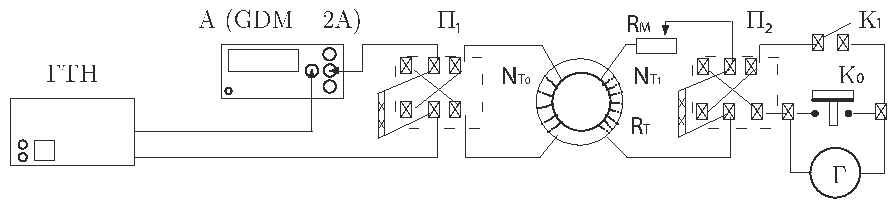
\includegraphics[scale = 1]{inst1.pdf}
		\end{figure}
		\begin{figure}[H]
			\caption{Схема установки для калибровки гальванометра}
			\label{inst2}
			\includegraphics[scale = 1]{inst2.pdf}
		\end{figure}
	\section*{Ход работы}
		\subsection*{Предельная петля гистерезиса}
			\begin{enumerate}
				\item Соберём схему по рисунку \ref{inst1}.
				\item Будем отмечать величину тока $ I $, соответствующею каждой ступени, и величину $ \Delta x $.
				\item Рассчитаем $ H $ и $ \Delta B $ по формулам:
				\begin{equation}\label{eq:1}
					H = \frac{N_{T_0}}{\pi D} I,
				\end{equation}
				\begin{equation}\label{eq:2}
					\Delta B = \mu_0 \left(\frac{d_C}{d_T}\right)^2 \frac{N_{C_0}}{N_{T_1}} \frac{N_{C_1}}{l_C} \Delta I_1 \frac{\Delta x}{\Delta x_1}.
				\end{equation}
			\end{enumerate}
		\subsection*{Калибровка гальванометра}
			\begin{enumerate}
				\item Соберём схему по рисунку \ref{inst2}.
				\item Измерим отклонение гальванометра $ \Delta x_1 $ при изменении тока $ \Delta I_1 = I_{max} $
				\item Данные занесём в таблицу \ref{table:D}.
			\end{enumerate}
		\subsection*{Начальная кривая намагничивания}
			\begin{enumerate}
				\item Размагнитим тороид в цепи переменного тока.
				\item Снимем начальную кривую намагничивания по той же схеме (рис. \ref{inst1}).
				\item Вычислим максимальное значение дифференциальной магнитной проницаемости $\mu_{диф}$:
				\begin{equation}
					\mu_{диф} = \frac{1}{\mu_0}\frac{dB}{dH}.
				\end{equation}
				\item Занесём параметры установки в таблицу \ref{table:D}.
			\end{enumerate}
			
	\section*{Обработка результатов}
		Полученные графики и таблицы представлены ниже:
		\begin{table}[H]
			\caption{Данные}
			\label{table:D}
			\begin{tabular}{|c|c|c|c|c|c|c|c|c|c|}
				\hline
				$N_{T_0}$ & $N_{T_1}$ & $N_{C_0}$ & $N_{C_1}$ & $D$, м & $d_C$, см & $d_T$, см & $l_C$, м & $\Delta x_1$, мм & $\Delta I_1$, А \\ \hline
				1750 & 300 & 940 & 500 & 0,1 & 7 & 1& 0,8 & 171 & 1,706 \\ \hline
			\end{tabular}
		\end{table}
		\begin{figure}[H]
			\caption{Зависимость $B$ от $H$}
			\label{ris:BH}
			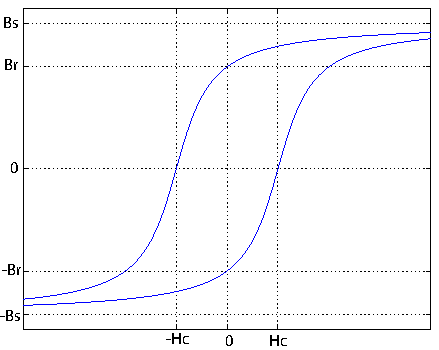
\includegraphics[scale = 0.7]{BH.pdf}
		\end{figure}
		\begin{table}[H]
			\caption{Вычисления}
			\label{table:Q}
			\begin{tabular}{|c|c|c|c|}
				\hline
				$H_C$, А/м & $B_S$, Тл  & $B_{ост}$, Тл & $\mu_{диф}$  \\ \hline
				$1600\pm 6$  & $1,41 \pm 0,01$ & $0,81\pm 0,01$ & $472 \pm 21$  \\ \hline
			\end{tabular}
		\end{table}
		
		\section*{Вывод}
			Таким образом, мы исследовали зависимость магнитной индукции от напряжённости магнитного поля для тороида из стали и вычислили коэрцитивную силу, индукцию насыщения, остаточную индукцию, а так же максимальное значение дифференциальной магнитной проницаемости.
			
\end{document} % конец документа

